\subsection{Morhpology and Filtering}

After isolating foreground objects it's necessary to remove noise and consolidate larger entities so that the only foreground pixels encountered by proceeding processes comprise vehicles. Because the GMM clusters pixels based on their value changes in lighting which might be caused by a cloud moving or a cars shadow among other others, can change the intensity of a background pixel and make it look like it's a foreground pixel. Furthermore, darker pixels, in car windows in particular, can make them appear like the road and hence background pixels, resulting in fractured foreground objects where only a single entitity should exist as in Figure \ref{fig:example_subtraction}.

\subsubsection{Filtering}

The noise generated by spurious foreground pixels looks a lot like salt and pepper noise and so to deal with this a median filter is applied to remove it (see Section \ref{subsection:median_filter}). The effect of this can be observed in Figure \ref{fig:foreground_mask_filtered}. It's important to remove this noise because it's evidently not a vehicle and will complicate proceeding image processing. 

\begin{figure*}[htbp]
    \centering 
    \begin{subfigure}[b]{0.45\textwidth}
        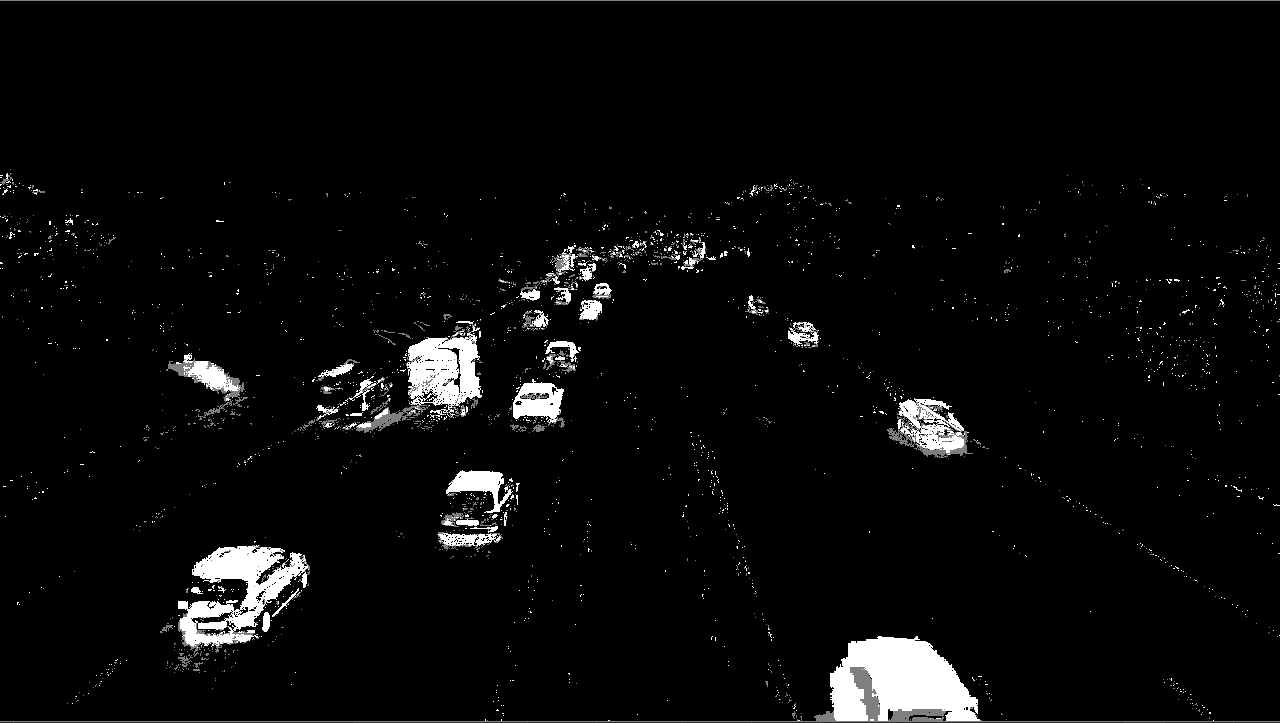
\includegraphics[width=\textwidth]{design/detection/subtractor/foreground_mask}
        \caption{Foreground mask generated by GMM clustering.}
    \end{subfigure}
    \begin{subfigure}[b]{0.45\textwidth}
        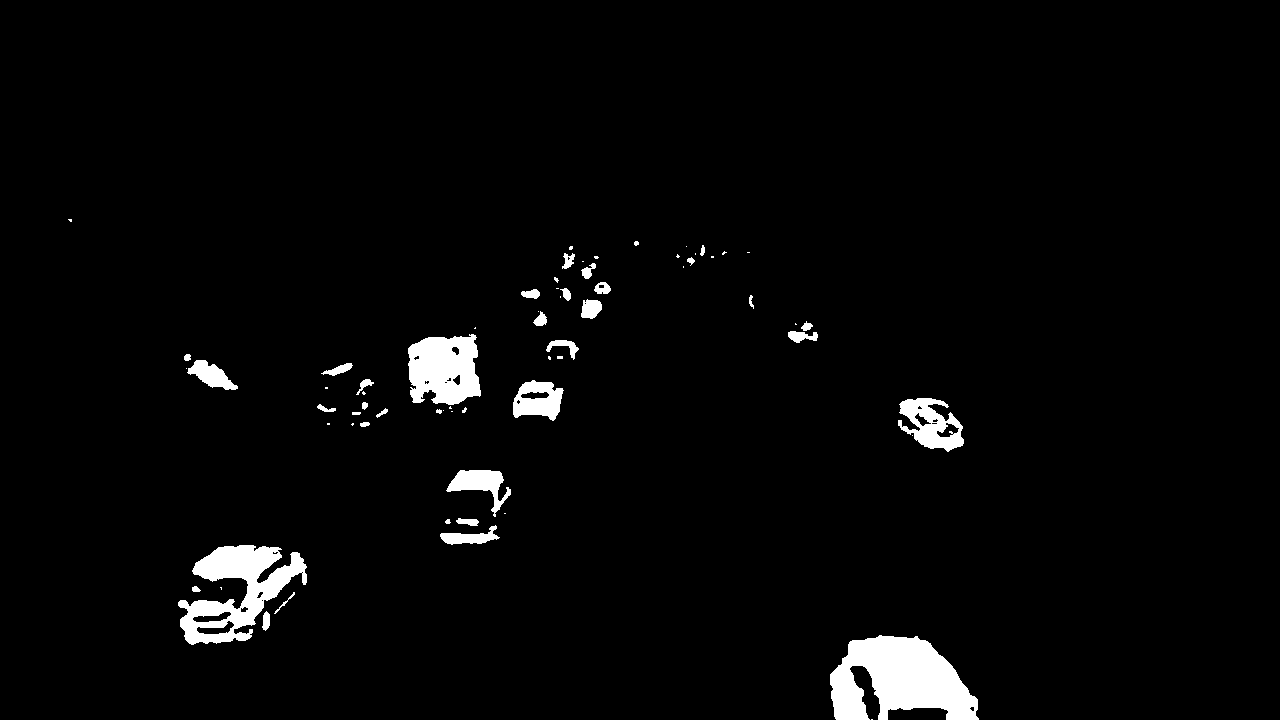
\includegraphics[width=\textwidth]{design/detection/morphology/foreground_mask_filtered}
        \captionsetup{format = hang}
        \caption{Foreground mask denoised by 5x5 median filter.}
    \end{subfigure}
    \captionsetup{format=hang}
    \caption{A foreground mask generated from a traffic scene by OpenCV's GMM implementation.}
    \label{fig:foreground_mask_filtered}
\end{figure*}

\subsubsection{Morphology}

The foreground objects that are presented at this point are mostly correct and whole however some are fractured due to their windows reflecting the same color as the road. To consolidate these fractured entities an opening, closing and dilation (section \ref{section:morphology}) are performed, as can be seen in Figure \ref{fig:foreground_mask_morphed}. 

\begin{figure*}[htbp]
    \centering 
    \begin{subfigure}[b]{0.45\textwidth}
        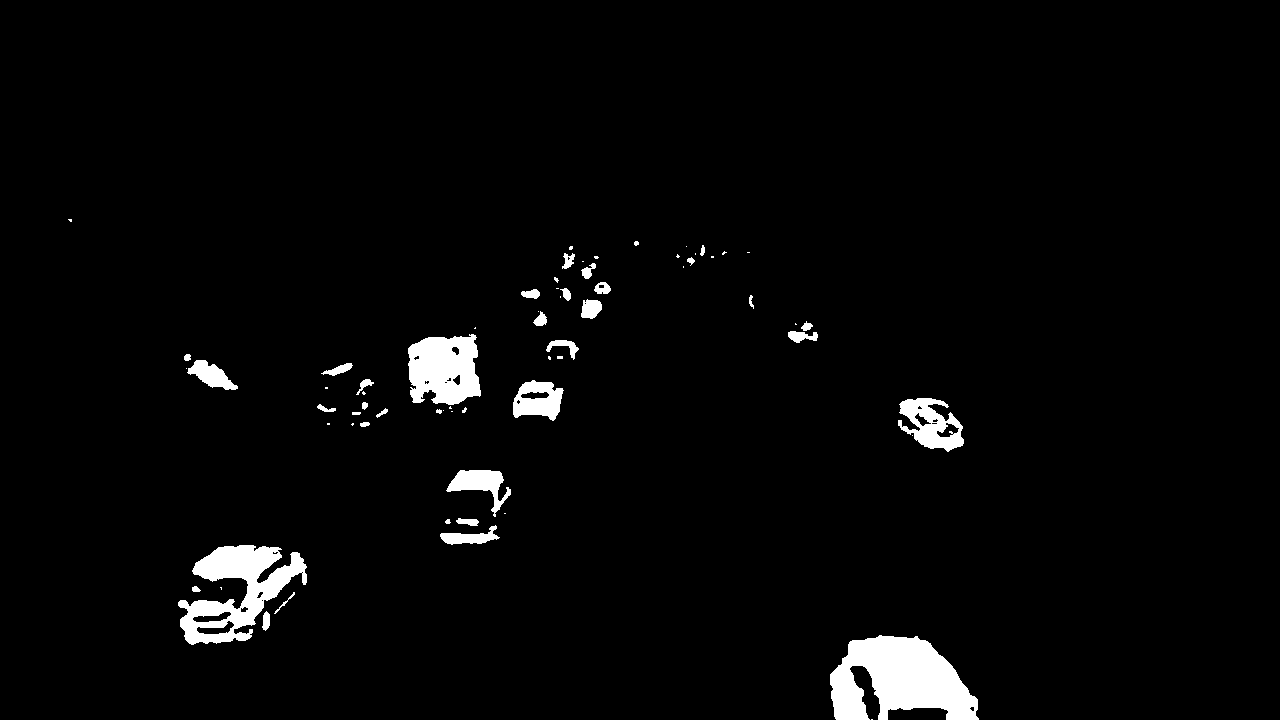
\includegraphics[width=\textwidth]{design/detection/morphology/foreground_mask_filtered}
        \captionsetup{format = hang}
        \caption{Foreground mask denoised by 5x5 median filter.}
    \end{subfigure}
    \begin{subfigure}[b]{0.45\textwidth}
        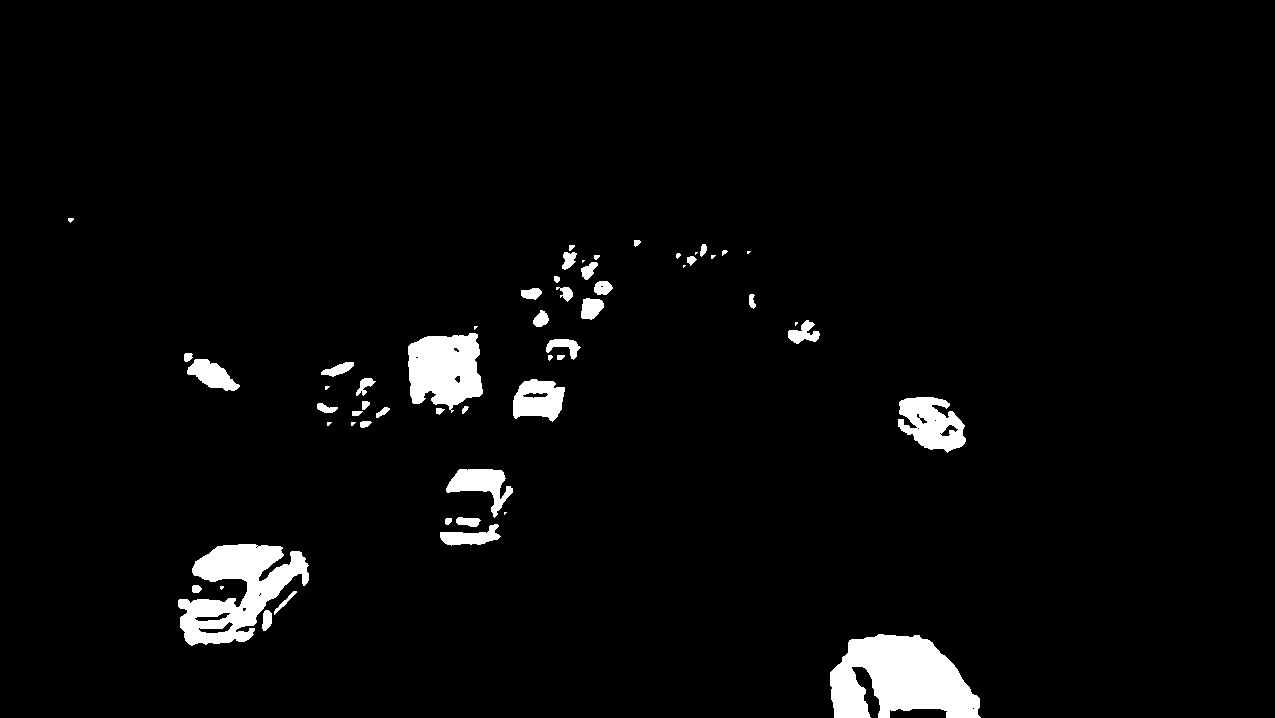
\includegraphics[width=\textwidth]{design/detection/morphology/foreground_mask_morphed}
        \captionsetup{format = hang}
        \caption{Foreground mask closed and dilated.}
    \end{subfigure}
    \captionsetup{format=hang}
    \caption{A foreground mask generated from a traffic scene by OpenCV's GMM implementation.}
    \label{fig:foreground_mask_morphed}
\end{figure*}

In determining the calibration of each 